
% Podstawowe definicje dla wszystkich dokumentów

\documentclass[12pt]{mwart}
%\setlength{\textwidth}{83pt}

\usepackage[OT4,plmath]{polski}
\usepackage{amsmath,amssymb,amsfonts,amsthm,mathtools}
\usepackage{color}
\usepackage{fontspec}
\usepackage{listings,times}

\usepackage{bbm}
\usepackage[colorlinks=false]{hyperref}
\usepackage{url}
\usepackage{graphicx}

\graphicspath{{images/}}

\newcommand{\HRule}{\rule{\linewidth}{0.5mm}}

\newcommand{\term}[1]{
  \indent\textbf{#1}
  \vspace{5pt}
}

\usepackage{multicol}

\usepackage{capt-of}

\usepackage{lmodern} \normalfont
%\DeclareFontShape{EU1}{ptm}{bx}{n} { <-> ssub * cmr/bx/n }{}
%\DeclareFontShape{EU1}{ptm}{m}{sc} { <-> ssub * cmr/m/sc }{}

%\usepackage{fancyhdr}
%\pagestyle{fancy}
%\fancyhead{}
%\fancyhead[LE,LO]{Iron Coach. \doctitle}
%\fancyhead[RO,RE]{\rightmark}
%\fancyfoot{}
%\fancyfoot[LE,RO]{}
%\fancyfoot[CO,CE]{\thepage}
%\addtolength{\headheight}{1.5pt}

\widowpenalty=10000
\clubpenalty=10000
\linepenalty=1000
\hyphenpenalty=10000
\raggedbottom

\renewcommand{\labelitemi}{}
\renewcommand{\labelitemii}{}
\renewcommand{\labelitemiii}{}
\renewcommand{\labelitemiv}{}

\newcommand{\titlep}[2] {
  \newcommand{\doctitle}{#1}
  \thispagestyle{empty}
  \begin{titlepage}
    \begin{center}
      \textsc{Studencka Pracownia Baz Danych}\\[0.5cm]
      \textsc{\large Instytut Informatyki\\Uniwersytetu Wrocławskiego}\\[1.5cm]


      \vspace{3.5cm}

      % Author and supervisor
      \begin{minipage}{\textwidth}
        \begin{center} \large
          Łukasz \textsc{Czapliński}
        \end{center}
      \end{minipage}

      \vspace{0.5cm}



      % Title
      \HRule \\[0.4cm]
      { \Large Dokumentacja projektu \\[0.5cm] }
      { \Huge \bfseries Coffee Shop  \\[1cm] }

      \textsc{\Large #1\\\large Wersja #2}\\[0.5cm]

      \HRule \\[1.5cm]

      \vspace{1cm}

      
      \vfill
      

      \vspace{1cm}

      % Bottom of the page
      {\large Wrocław 2014}

    \end{center}
  \end{titlepage}
  \clearpage
  \setcounter{page}{2}
}

\newcommand{\chist}[1]{
  \begin{table}
  \centering
  \caption{Historia zmian}
  \begin{tabular}{l | l | p{5cm} | p{5cm}}
    Wersja & Data & Opis & Autor \\ 
    \hline
    \noalign{\smallskip}
    #1
  \end{tabular}
\end{table}
}


\begin{document}
\titlep{Instrukcja dla użytkownika -- klient}{1.0}
\chist{1.0 & 2014-06-13 & Powstanie dokumentu & Łukasz Czapliński\\
        }
\tableofcontents
\clearpage
\section{Wprowadzenie}
\subsection{Cel dokumentu}
Dokument ten ma na celu pokazanie, jakie możliwości otwiera przed klientem aplikacja Coffee Shop.
\section{Nawigacja}
Nawigowanie w aplikacji odbywa się poprzez klawisze: TAB, ESCAPE, ENTER i strzałki. \begin{itemize}
  \item[TAB] -- pozwala na przełączanie się pomiędzy różnymi elementami (listami, przyciskami, itd). Odbywa się to w sposób cykliczny -- po dostatecznej ilości naciśnięć aktywny będzie ponownie pierwszy element.
  \item[ENTER] -- zatwierdza wybór (aktywuje zaznaczony na biało element).
  \item[ESCAPE] -- pozwala natychmiast wyjść porzucając pracę.
  \item[strzałki] -- dają możliwość aktywnego elementu w liście.
\end{itemize}
Przycisk "Back" na każdej stronie pozwala wrócić na stronę, z której przyszedłeś do aktualnej po raz pierwszy.
\section{Kupujący}
\subsection{Ekran powitalny}
Po uruchomieniu aplikacji Coffee Shop zawsze będziesz powitany przez taki ekran. Możesz z niego przejść do ekranu logowania ($\rightarrow$[\ref{log}]) poprzez aktywację przycisku "Logowanie" lub wyjść używając przycisku "Back".
\label{pow}
\begin{figure}
  \centering
  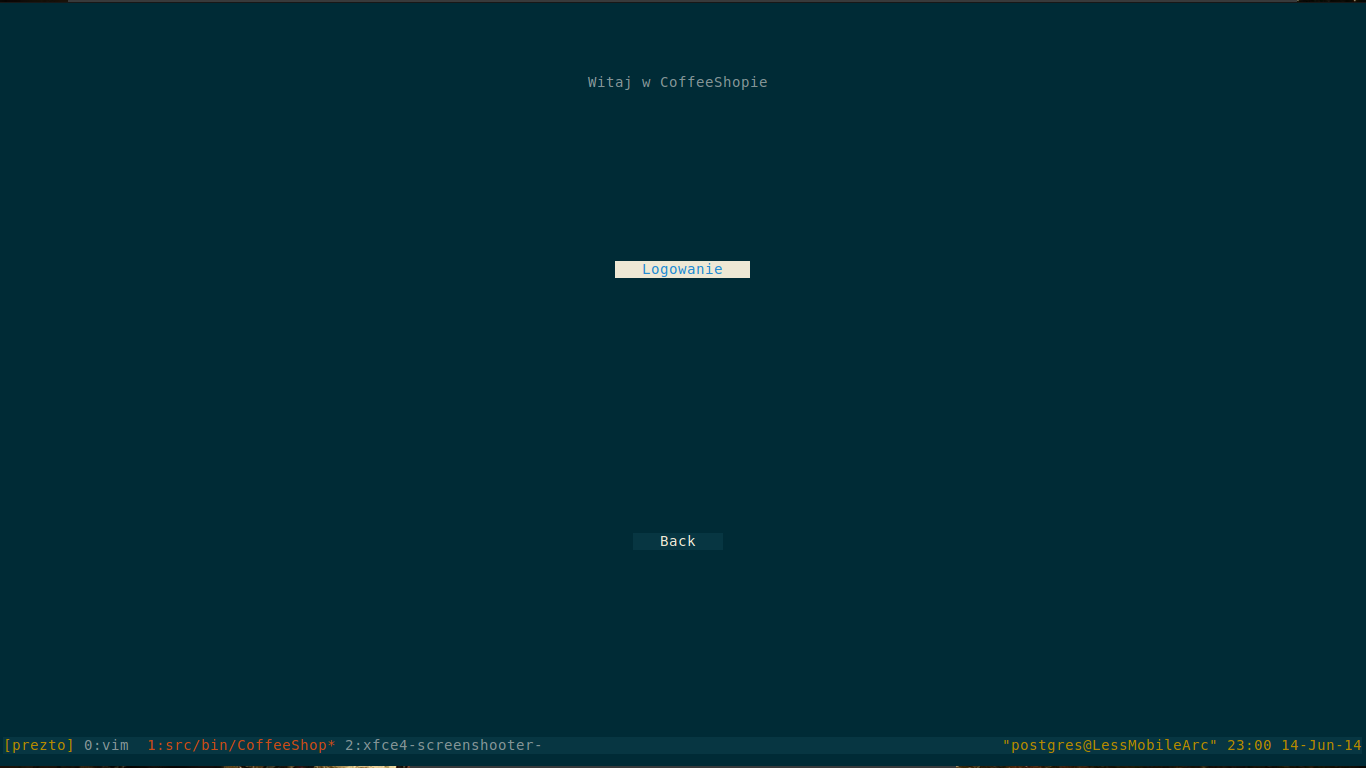
\includegraphics[width=0.95\textwidth]{pow.png}
  \caption{Ekran logowania: [\ref{pow}]}
  \label{powI}
\end{figure}
\subsection{Ekran logowania}
Używając strzałek należy wybrać opcję "Kupujący" ($\rightarrow$[\ref{logId}]) lub cofnąć się przyciskiem "Back".
\label{log}
\begin{figure}
  \centering
  \includegraphics[width=0.95\textwidth]{log.png}
  \caption{Ekran logowania: [\ref{log}]}
  \label{logI}
\end{figure}
\subsubsection{Podaj id}
\label{logId}
Tutaj należy wpisać swoje id -- każdy klient otrzymuje od Administratora unikalny identyfikator, którego powinien używać podczas korzystania z aplikacji Coffee Shop. Po wpisaniu przycisk "Ok" przeniesie do ekranu głównego ($\rightarrow$[\ref{głó}]). W przypadku podania złego identyfikatora pojawi się ekran błędu.
\begin{figure}
  \centering
  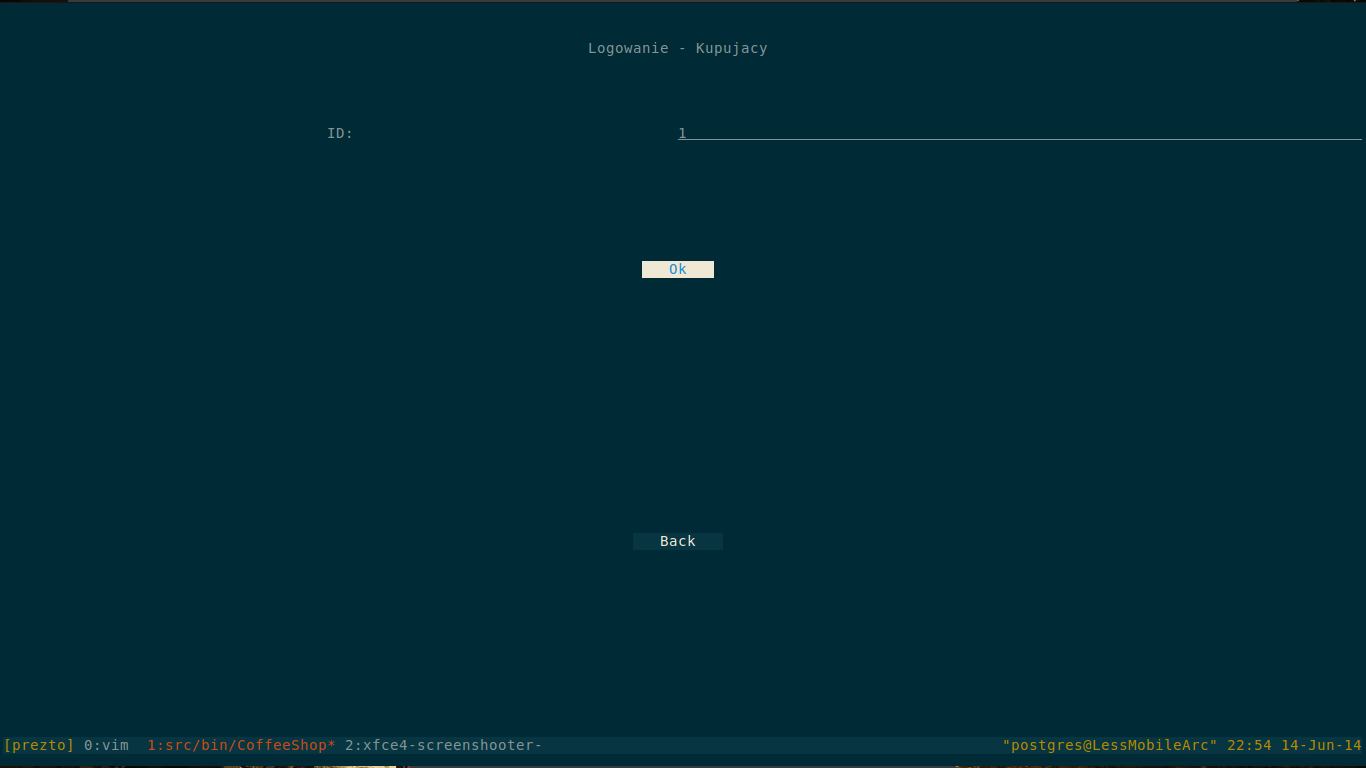
\includegraphics[width=0.95\textwidth]{logId.png}
  \caption{Podaj swoje id}
  \label{logIdI}
\end{figure}
\subsection{Ekran główny}
\label{głó}
Można się z niego przenieść do ekranów: 
\begin{itemize}[leftmargin=5cm]
\item["Historia zamówień"]($\rightarrow$[\ref{hzam}]), 
\item["Zobacz produkty"]($\rightarrow$[\ref{zpr}]), który pozwala na zamówienie produktu, 
\item["Zobacz sprzedawców"]($\rightarrow$[\ref{zsp}]), który pozwala na dodanie zamówienia,
\item["Zobacz niezłożone zamówienia"]($\rightarrow$[\ref{znz}]), który pozwala na złożenie zamówienia.
\end{itemize}
\begin{figure}
  \centering
  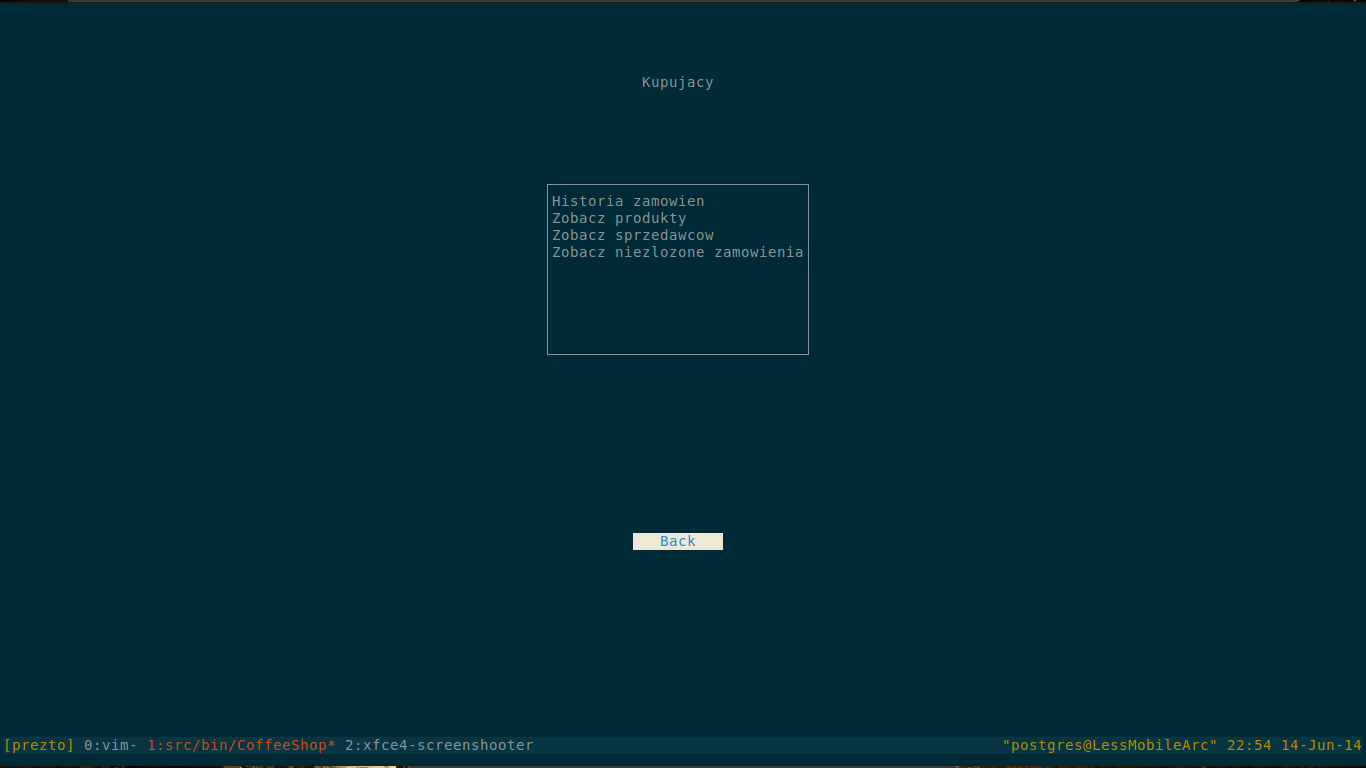
\includegraphics[width=0.95\textwidth]{głó.png}
  \caption{Ekran główny: [\ref{głó}]}
  \label{głóI}
\end{figure}
\subsection{Historia zamówień}
\label{hzam}
Ekran ten pokazuje wszystkie Twoje zamówienia.
Wybranie zamówienia skutkuje przeniesieniem do ekranu szczegółów zamówienia ($\rightarrow$[\ref{szam}]).
\begin{figure}
  \centering
  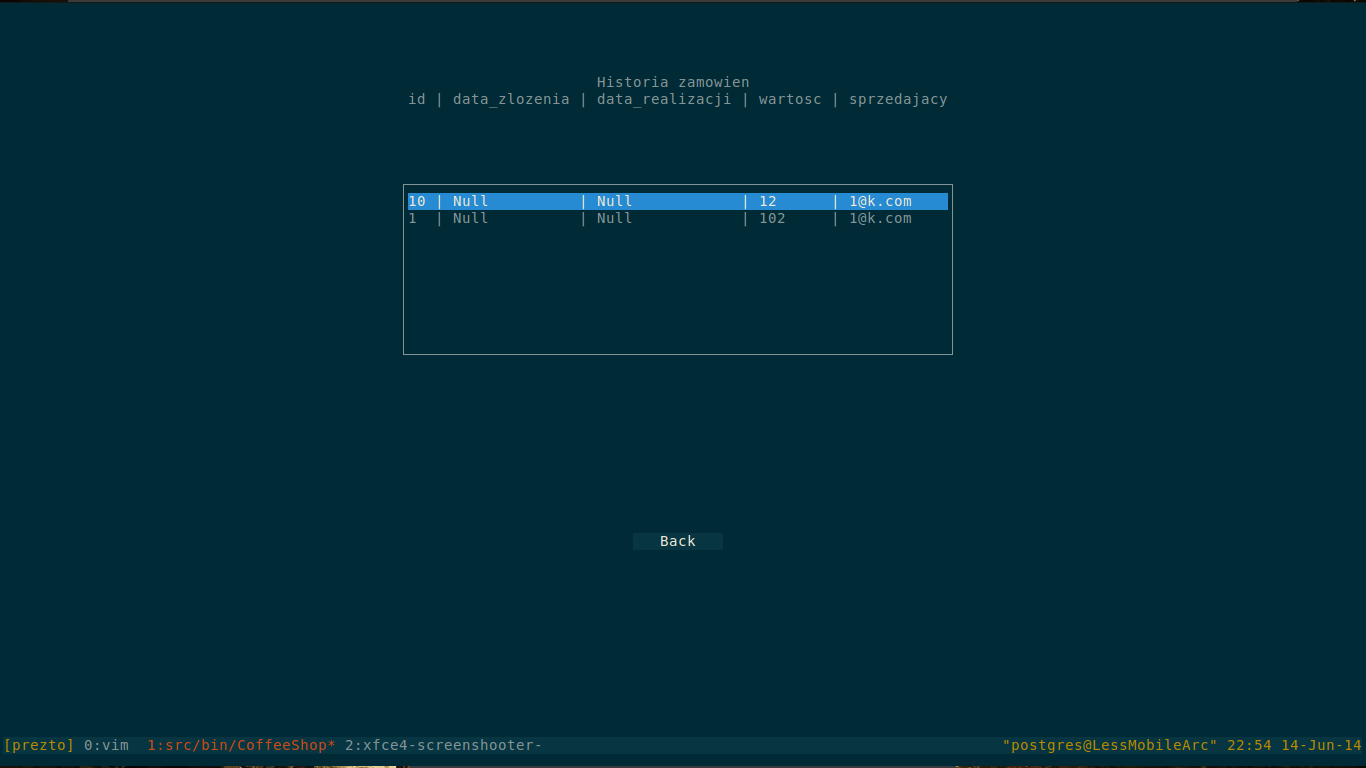
\includegraphics[width=0.95\textwidth]{hzam.png}
  \caption{Historia zamówień: [\ref{hzam}]}
  \label{hzamI}
\end{figure}
\subsection{Szczegóły zamówienia}
\label{szam}
Ekran ten pokazuje wszystkie produkty, jakie znalazły się w danym zamówieniu.
\begin{figure}
  \centering
  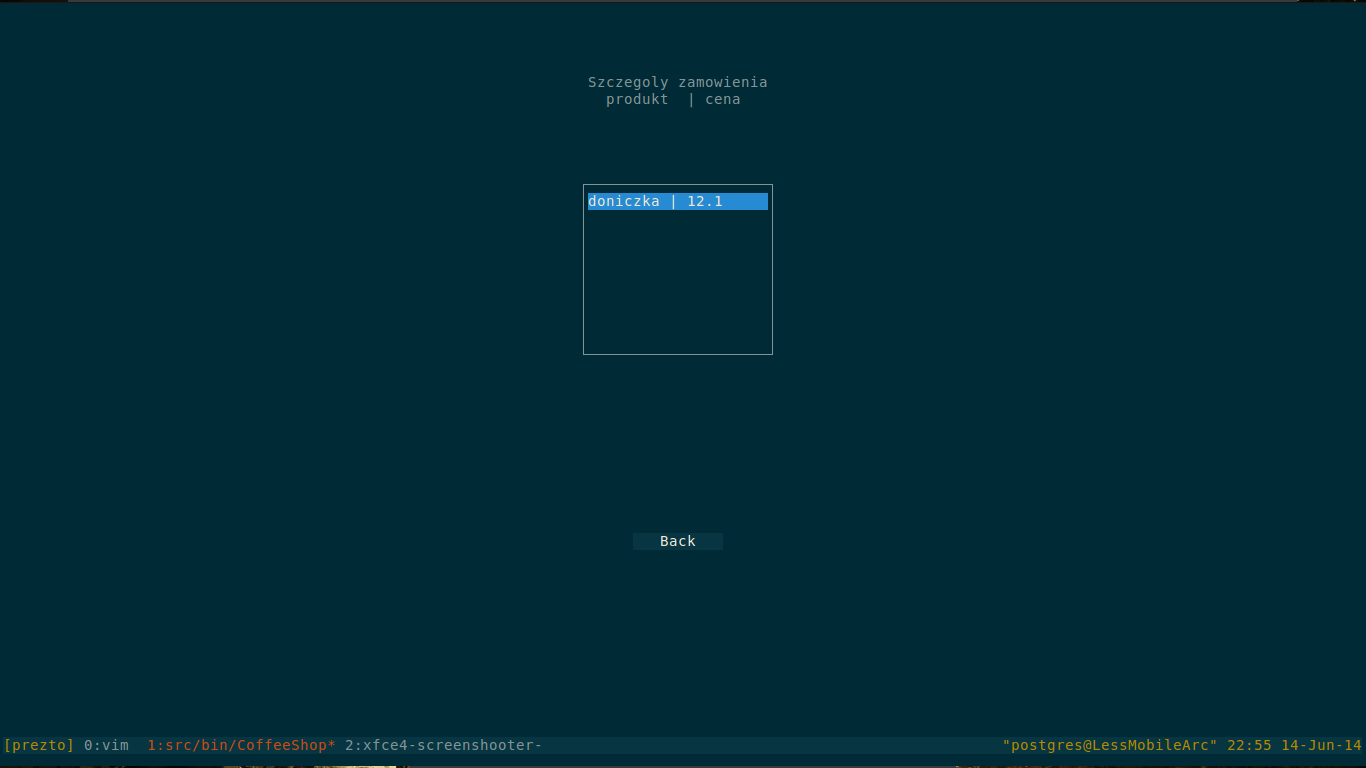
\includegraphics[width=0.95\textwidth]{szam.png}
  \caption{Szczegóły zamówienia: [\ref{szam}]}
  \label{szamI}
\end{figure}
\subsection{Zobacz produkty}
\label{zpr}
Pokazuje wszystkie typy produktów, jakie wszyscy właściciele mają w magazynach. Po wybraniu typu produktu zostaniesz przeniesiony do ekranu "Właściciele produktów" ($\rightarrow$[\ref{wpr}]), który pozwoli Ci na wybór najlepszego produktu danego typu i zamówienie go.
\begin{figure}
  \centering
  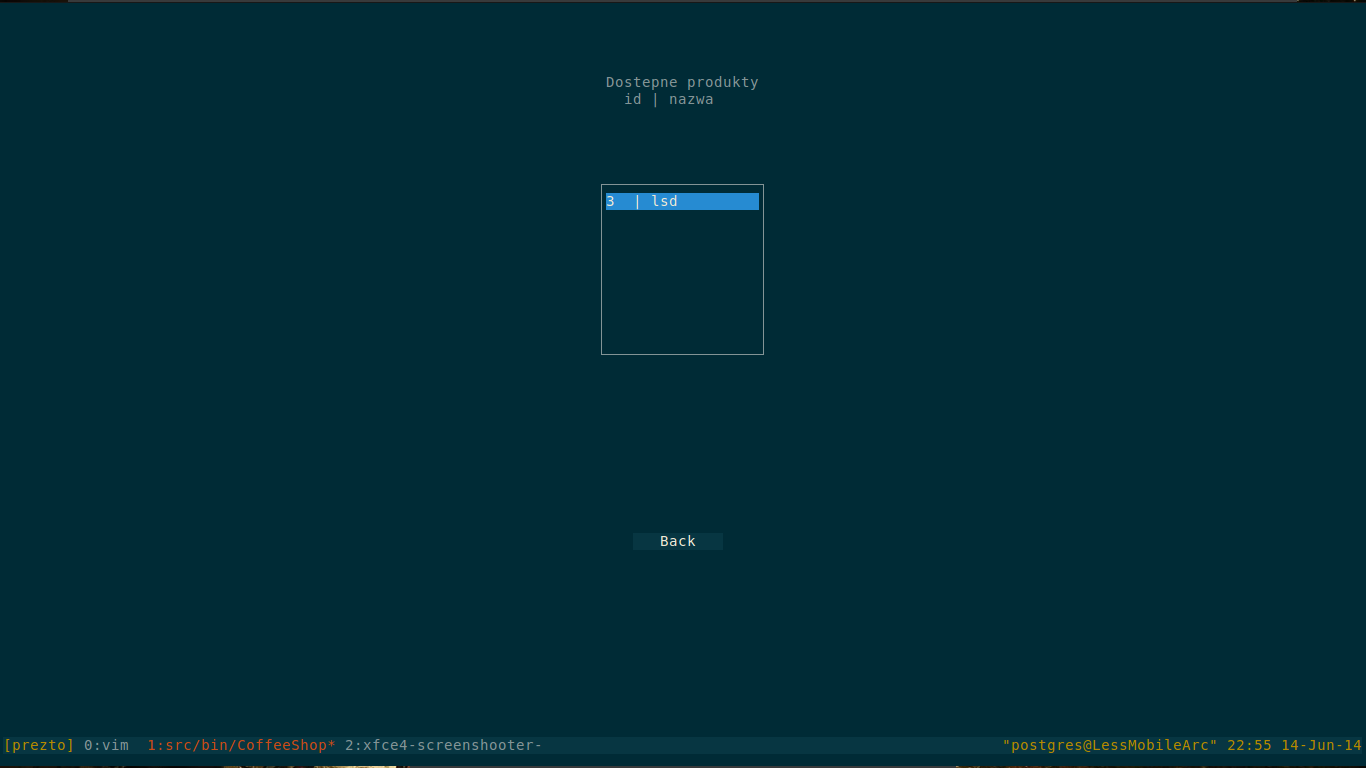
\includegraphics[width=0.95\textwidth]{zpr.png}
  \caption{Zobacz produkty: [\ref{zpr}]}
  \label{zprI}
\end{figure}
\subsection{Właściciele produktów}
Ekran ten pokazuje kto ma dany typ produktu i w jakiej cenie go oferuje. Wybór konkretnego produktu przenosi do ekranu~[\ref{dzam}].
\label{wpr}
\begin{figure}
  \centering
  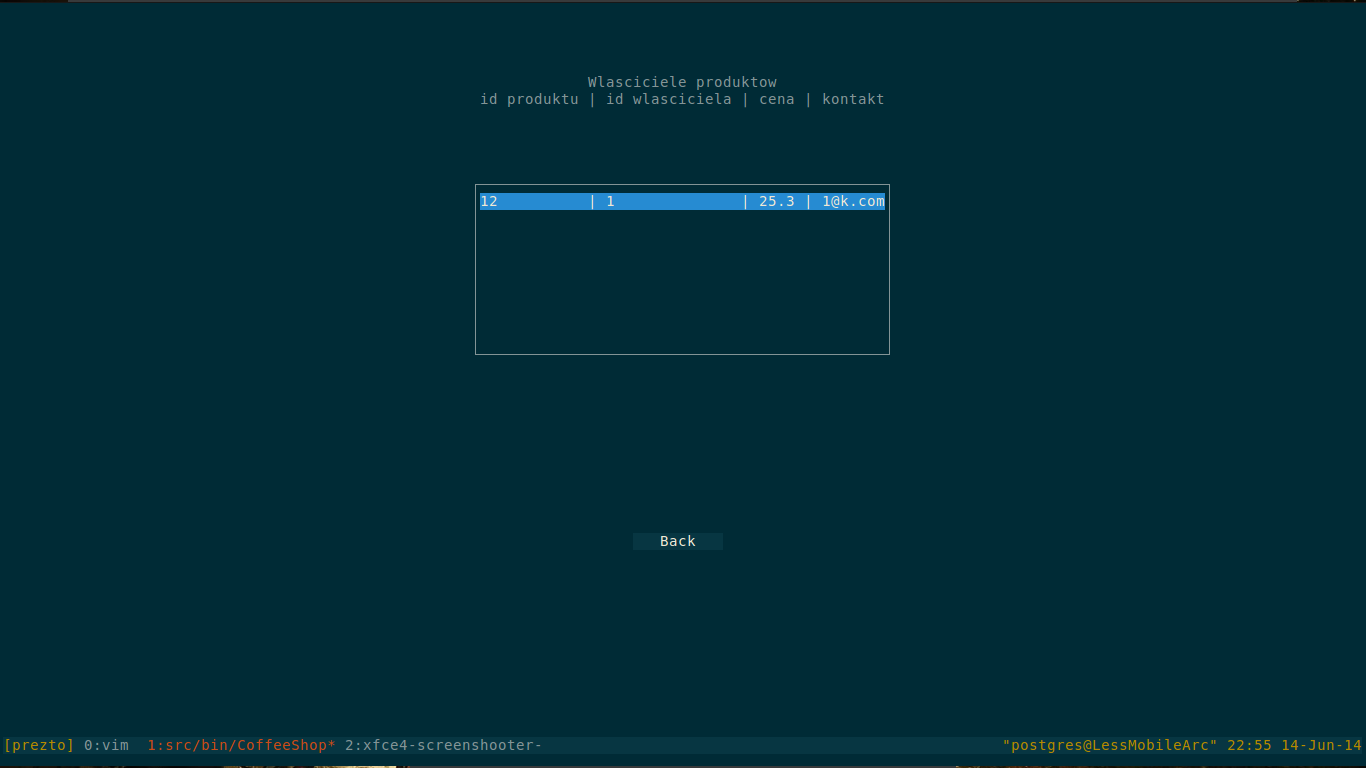
\includegraphics[width=0.95\textwidth]{wpr.png}
  \caption{Właściciele produktów: [\ref{wpr}]}
  \label{wprI}
\end{figure}
\subsection{Dodaj do zamówienia}
Ekran ten pozwala wybrać do jakiego zamówienia chcemy dodać dany produkt. Jeśli nie ma takiego zamówienia, to należy je złożyć poprzez opcję "Zobacz sprzedawców" w ekranie głównym ($\rightarrow$[\ref{głó}]).
\label{dzam}
\begin{figure}
  \centering
  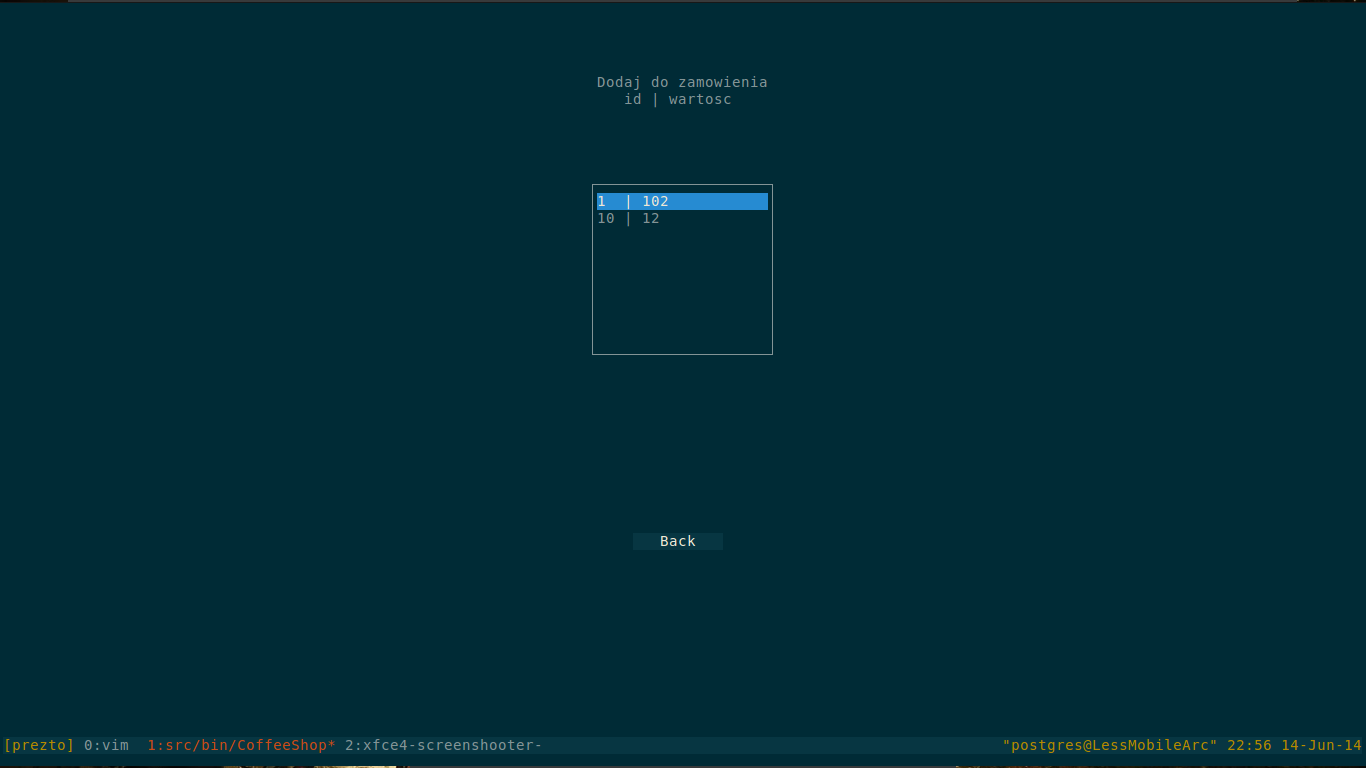
\includegraphics[width=0.95\textwidth]{dzam.png}
  \caption{Dodaj do zamówienia: [\ref{dzam}]}
  \label{dzamI}
\end{figure}
\subsection{Zobacz sprzedawców}
\label{zsp}
Pokazuje listę wszystkich sprzedawców oraz ilość naszych niezłożonych zamówień u każdego z nich. Wybór jednego ze sprzedawców pozwoli na dodanie nowego zamówienia do niego.
\begin{figure}
  \centering
  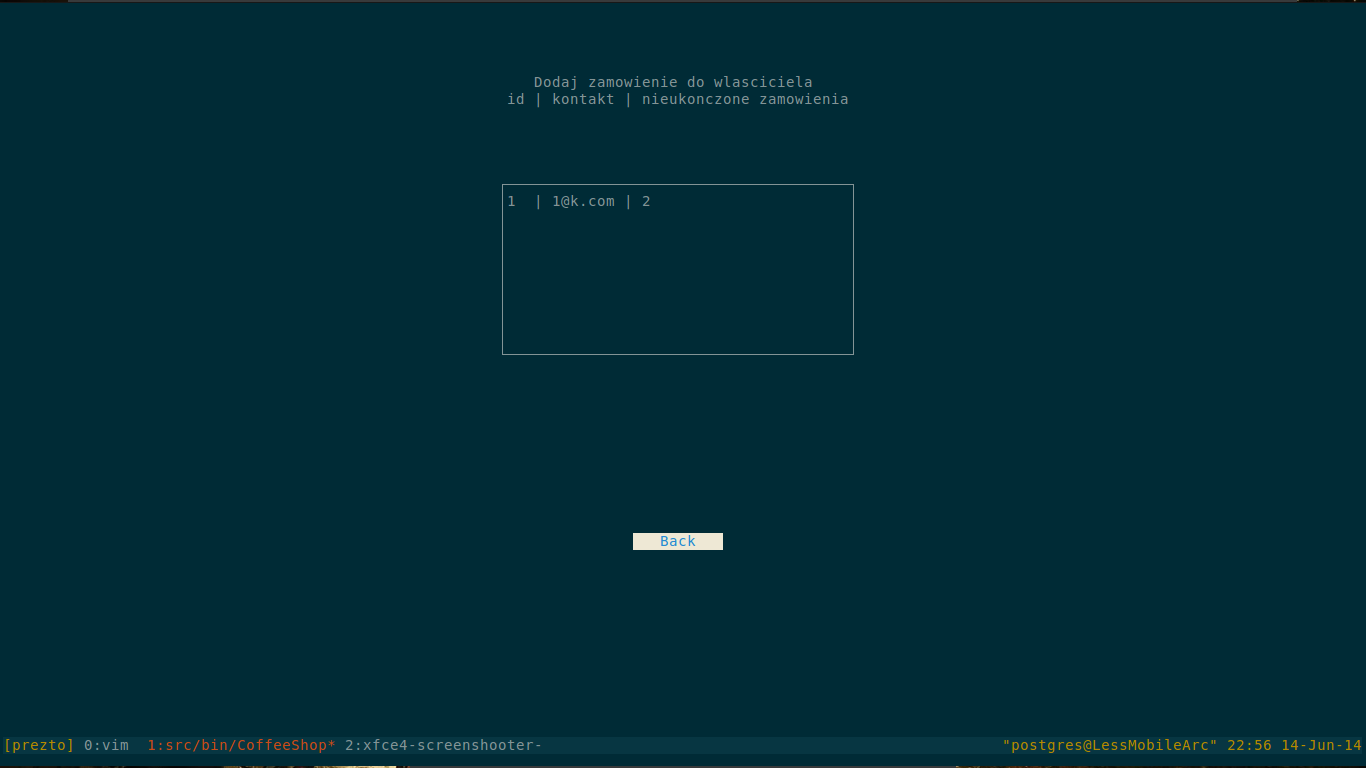
\includegraphics[width=0.95\textwidth]{zsp.png}
  \caption{Zobacz sprzedawców: [\ref{zsp}]}
  \label{zspI}
\end{figure}
\subsection{Zobacz niezłożone zamówienia}
Pokazuje wszystkie nasze niezłożone zamówienia. Wybór jednego pozwoli na złożenie go.
\label{znz}
\begin{figure}
  \centering
  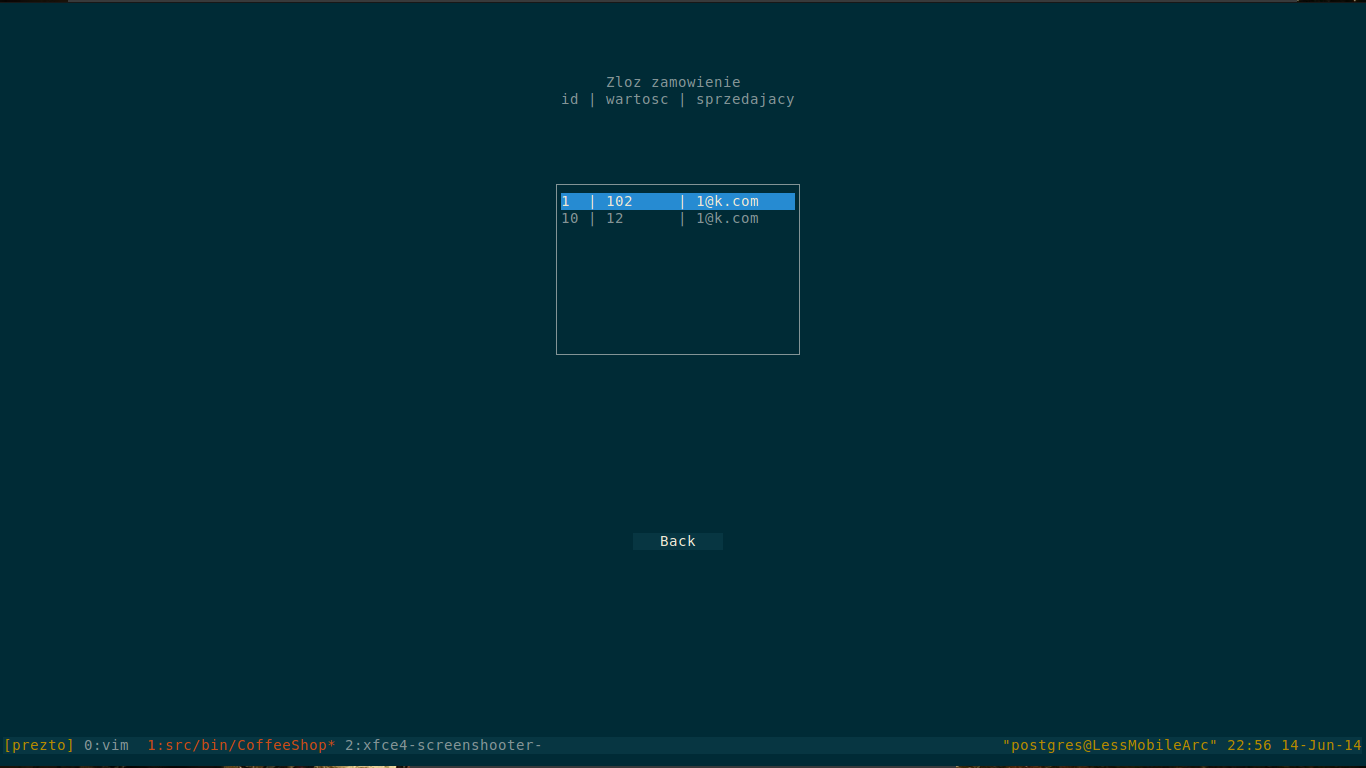
\includegraphics[width=0.95\textwidth]{znz.png}
  \caption{Zobacz niezłożone zamówienia: [\ref{znz}]}
  \label{znzI}
\end{figure}
\end{document}
